% capitulos/cap3.tex — Capítulo 3 (Metodologia).
% Reescrito em 25/09/2026 no enxugamento pós-feedback (ver
% auditoria/plano_enxugamento.md). Mudanças em relação à versão de
% 29/08/2026 (auditoria/versoes/pre_enxugamento/cap3.tex):
% (1) a antiga seção 3.1 (fluxo atual e os cinco elementos E1-E5) migrou,
%     condensada, para o Capítulo 2 — a Metodologia começa direto no método;
% (2) os oito passos viram seções numeradas em sequência, sem subseções
%     soltas entre eles ("Cenário pretendido" e "Estratégia de avaliação"
%     foram absorvidas por 3.1 e pelo Passo 3);
% (3) siglas reduzidas: E1-E5, I1-I6, C0/C1 e "1e" saem do texto; ficam
%     R1-R5 e, só no quadro próprio, S1-S5;
% (4) limitações reunidas em uma seção única (3.11);
% (5) detalhes cortados ficam guardados para o TG2 (índice em
%     auditoria/plano_enxugamento.md, seção 4).
% Contém: 9 Quadros (eram 14), 1 Tabela, 2 Figuras (fig:fluxo-metodologico,
% fig:to-be; fig4_arquitetura e fig5_sintese retiradas). As equações
% eq:pl/eq:milp passaram para o Capítulo 2.
\chapter{Metodologia}

Este capítulo descreve como a pesquisa será conduzida. A seção~\ref{sec:dsr} caracteriza a pesquisa e apresenta o caminho metodológico, organizado pela \textit{Design Science Research} em oito passos. As seções~\ref{sec:requisitos-projeto} a~\ref{sec:falhas} descrevem os passos na ordem em que são executados; cada um usa o produto do anterior e entrega o que o seguinte precisa. A seção~\ref{sec:piloto} relata o piloto feito nesta etapa, e a seção~\ref{sec:limitacoes} reúne as limitações do desenho.

\section{Caracterização da pesquisa e caminho metodológico}
\label{sec:dsr}

A pesquisa é aplicada quanto à natureza, pois constrói um artefato para um problema organizacional específico; exploratória quanto aos objetivos; quantitativa na etapa de avaliação; e combina pesquisa bibliográfica e experimento quanto aos procedimentos.

O método condutor é a \textit{Design Science Research} (DSR), nas seis etapas de \citeonline{peffers2007}: identificação do problema e motivação, definição dos objetivos da solução, projeto e desenvolvimento, demonstração, avaliação e comunicação. A DSR é o único método do trabalho. A revisão de literatura, a construção do artefato, a demonstração e o experimento são os instrumentos com que cada etapa é realizada. A Figura~\ref{fig:fluxo-metodologico} mostra os oito passos em sequência, e o Quadro~\ref{q:dsr} indica a que etapa da DSR cada passo pertence, o que ele produz e como esse produto é usado adiante.

\begin{figure}[htbp]
\caption{Caminho metodológico: os oito passos e o que cada um produz}
\label{fig:fluxo-metodologico}
\centering
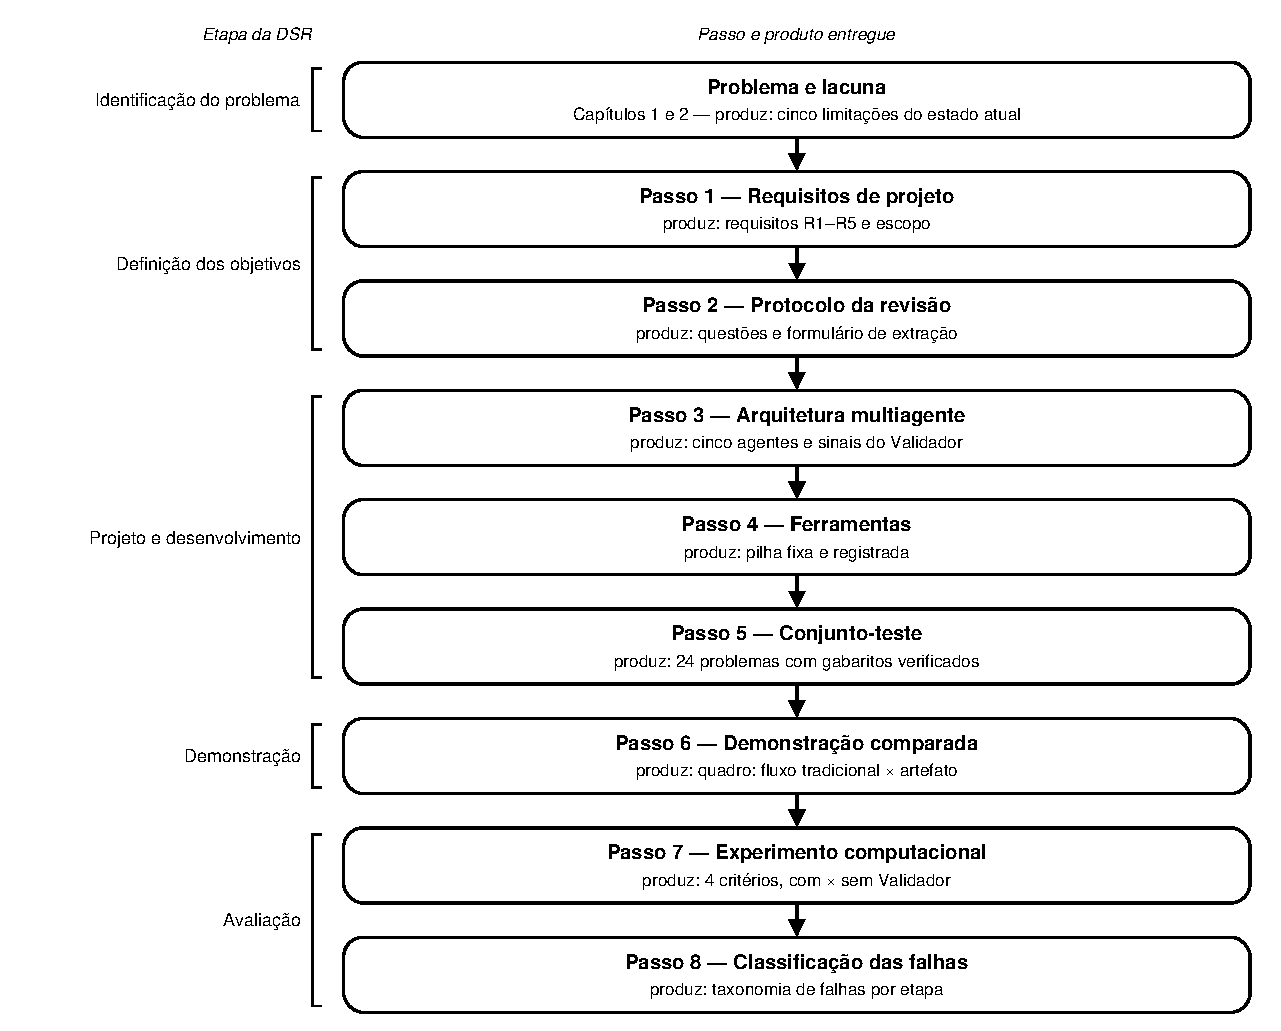
\includegraphics[width=0.9\textwidth]{figuras/fig2_fluxo_metodologico.pdf}
\fontenota{elaborado pelo autor}
\end{figure}

\begin{quadro}[htbp]
\caption{Etapas da DSR e sua realização no trabalho}
\label{q:dsr}
\centering
\small
\begin{tabularx}{\textwidth}{@{}X l X X@{}}
\toprule
Etapa da DSR & Passos & Produto & Uso na etapa seguinte \\
\midrule
Identificação do problema & Caps. 1 e 2 & Cinco limitações do estado atual & Convertidas em requisitos no Passo 1 \\
Definição dos objetivos & 1 e 2 & Requisitos R1--R5; protocolo da revisão & Orientam o desenho da arquitetura \\
Projeto e desenvolvimento & 3, 4 e 5 & Arquitetura, ferramentas e conjunto-teste de 24 problemas & Insumo comum da demonstração e do experimento \\
Demonstração & 6 & Quadro comparativo entre o fluxo tradicional e o artefato & Falhas observadas alimentam o Passo 8 \\
Avaliação & 7 e 8 & Resultados dos quatro critérios; classificação das falhas & Conclusões e trabalhos futuros \\
Comunicação & --- & Documento e apresentação à banca & --- \\
\bottomrule
\end{tabularx}
\fontenota{elaborado pelo autor com base em \citeonline{peffers2007}}
\end{quadro}

No TG1, os Passos 1 a 5 são especificados e um piloto verifica a viabilidade técnica (seção~\ref{sec:piloto}); a construção do artefato e a execução dos Passos 6 a 8 ocorrem no TG2. Os critérios de avaliação são definidos antes da construção porque, na DSR, os objetivos da solução precedem o projeto. Isso também impede que os critérios sejam ajustados depois, conforme o que o artefato conseguir fazer.

Para posicionar a avaliação, adota-se o arcabouço FEDS \cite{venable2016}, na estratégia \textit{Technical Risk \& Efficacy}. Ela é indicada quando o principal risco é técnico e quando é preciso mostrar com rigor que o efeito observado vem do artefato, e não de outro fator \cite[p.~82]{venable2016}. É o caso do experimento, que isola o efeito do agente Validador em ambiente controlado. A demonstração comparada, por sua vez, pertence à etapa de Demonstração da DSR: aplica o artefato a casos concretos e não é um experimento. Sua unidade de análise é o caso resolvido, e não a pessoa que o resolveu.

\section{Passo 1: requisitos de projeto}
\label{sec:requisitos-projeto}

As cinco limitações do estado atual (seção~\ref{sec:lacunas}) convertem-se em cinco requisitos de projeto. O Quadro~\ref{q:requisitos} apresenta cada requisito e onde ele é aferido.

\begin{quadro}[htbp]
\caption{Requisitos de projeto e ponto de aferição}
\label{q:requisitos}
\centering
\small
\begin{tabularx}{\textwidth}{@{}l X l X@{}}
\toprule
Req. & Enunciado & Limitação & Onde é aferido \\
\midrule
R1 & Conduzir a decisão sem exigir do usuário conhecimento de Pesquisa Operacional & Usuário & Demonstração: pré-requisitos e tempo \\
R2 & Percorrer o fluxo completo, da interpretação à explicação, sem intervenção externa & Fluxo completo & Experimento: critério 2; demonstração: ferramentas, etapas e tempo \\
R3 & Obter e associar parâmetros de fontes externas de dados estruturados, pedindo ao usuário o tratamento que faltar & Dados & Experimento: acurácia da associação e critério 2 \\
R4 & Conduzir a interação em língua portuguesa & Idioma & Condição de todo o protocolo \\
R5 & Expor premissas, componentes matemáticos, validações e alterações do processo & Rastreabilidade & Demonstração: relatórios e rastreabilidade; experimento: critério 4 \\
\bottomrule
\end{tabularx}
\fontenota{elaborado pelo autor}
\end{quadro}

O agente Validador não é um sexto requisito: é o mecanismo que realiza R5. Para que as validações e correções fiquem expostas, alguém precisa produzi-las e registrá-las, e esse é o papel do Validador. Como ele é um componente separável, seu efeito pode ser medido, o que transforma uma escolha de arquitetura em hipótese testável (critério 4, seção~\ref{sec:experimento}). É o experimento que os autores do OptiAgent deixaram como trabalho futuro \cite[p.~11]{monteiro2026}.

Com isso, a pergunta de pesquisa fica coberta em duas partes. A primeira --- se a arquitetura produz modelos corretos, executáveis e rastreáveis --- é respondida pelos critérios 1 a 3 do experimento e pela demonstração comparada. A segunda --- qual o efeito do agente validador --- é respondida pelo critério 4.

O escopo é o seguinte: problemas de PL e PLIM em três famílias (alocação de recursos, mistura de insumos e transporte ou distribuição), em organizações que atendem às condições de aplicabilidade da PO descritas na seção~\ref{sec:po-barreira}. Ficam fora problemas não lineares, formulações estocásticas, uso por vários usuários simultâneos e operação em escala de produção.

\section{Passo 2: protocolo da revisão de literatura}
\label{sec:revisao}

A revisão sistemática confirma a lacuna e levanta as arquiteturas concorrentes, informando as decisões do Passo 3; seus resultados ampliarão o Capítulo 2 no TG2. O processo segue as diretrizes de \citeonline{kitchenham2007}, e o relato segue o PRISMA 2020 \cite{page2021}. As questões de revisão são:

\begin{enumerate}[label=QR\arabic*.]
  \item Quais arquiteturas baseadas em modelos de linguagem foram propostas para formular e resolver problemas de otimização, e que etapas do fluxo de modelagem cada uma cobre?
  \item Qual é o público-alvo declarado dessas arquiteturas, e que conhecimento prévio elas pressupõem do usuário?
  \item De onde vêm os parâmetros dos modelos, e em que medida as fontes de dados existem antes do modelo?
  \item Que mecanismos de validação, correção e rastreabilidade essas arquiteturas incorporam, e como seu efeito é avaliado?
\end{enumerate}

No planejamento, definem-se as bases, as expressões de busca e a janela temporal, a partir de 2022. Na condução, aplicam-se critérios de inclusão e exclusão fixados de antemão, com triagem por título e resumo e depois por texto completo. A extração registra, para cada trabalho, uma coluna por limitação da seção~\ref{sec:lacunas}, além da classe de problema, do tipo de avaliação e do número de repetições por instância. O relato traz o fluxograma PRISMA e um quadro comparativo dos trabalhos incluídos. A ferramenta Elicit apoia a triagem e a extração, com conferência manual de todos os itens.

\section{Passo 3: arquitetura multiagente}
\label{sec:arquitetura}

O artefato é um encadeamento de cinco agentes especializados sobre um estado compartilhado. Cada agente recebe uma entrada definida, produz uma saída definida e registra ao menos um artefato que o usuário pode inspecionar. Cada um assume um estágio do fluxo atual de modelagem (seção~\ref{sec:po-barreira}), como mostram a Figura~\ref{fig:to-be} e o Quadro~\ref{q:agentes}.

\begin{figure}[htbp]
\caption{Cenário \textit{to be}: fluxo de modelagem mediado pela plataforma multiagente}
\label{fig:to-be}
\centering
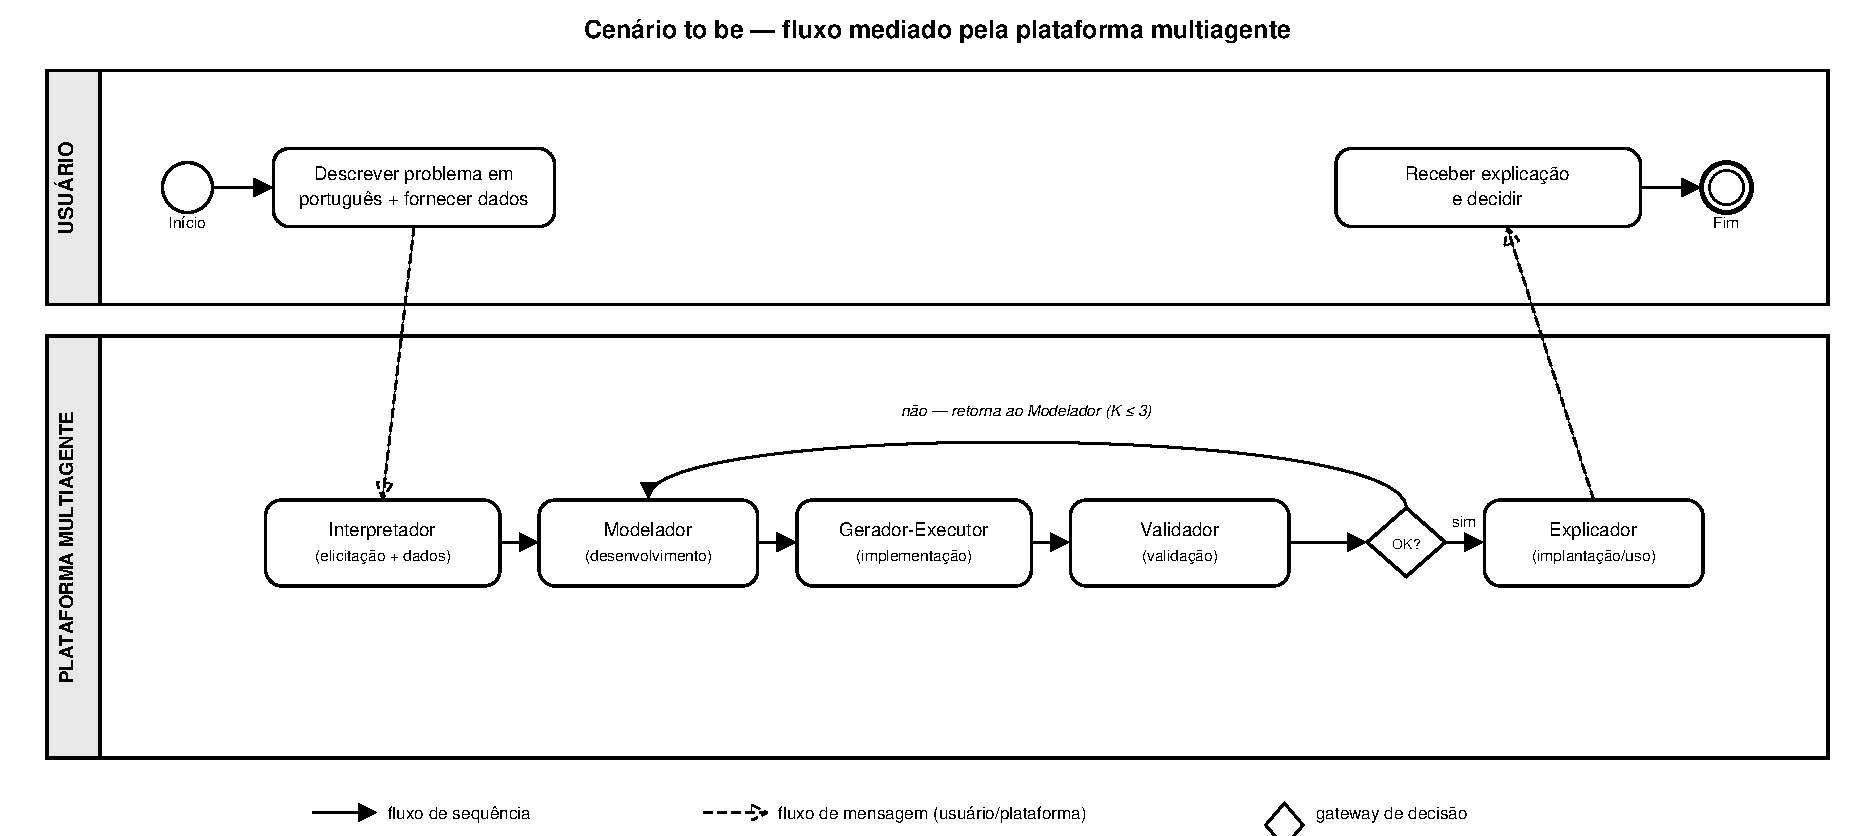
\includegraphics[width=0.95\textwidth]{figuras/fig3_to_be.pdf}
\fontenota{elaborado pelo autor}
\end{figure}

\begin{quadro}[htbp]
\caption{Agentes: estágio assumido, entrada, saída e artefato registrado}
\label{q:agentes}
\centering
\small
\begin{tabularx}{\textwidth}{@{}l X X X@{}}
\toprule
Agente & Estágio do fluxo atual & Entrada $\rightarrow$ saída & Artefato registrado \\
\midrule
Interpretador & Elicitação e tratamento dos dados & Descrição e fontes de dados $\rightarrow$ quadro de especificação & Lista de requisitos; inventário das fontes; solicitações de tratamento e respostas; alertas de ambiguidade \\
Modelador & Desenvolvimento do modelo & Quadro de especificação $\rightarrow$ modelo em JSON & Documento JSON, com o requisito de origem de cada restrição \\
Gerador-Executor & Implementação & JSON $\rightarrow$ código e resultado & Script e registro de execução do \textit{solver} \\
Validador & Validação & JSON, quadro e resultado $\rightarrow$ aprovação ou erro localizado & Registro das validações, com o sinal que originou cada uma \\
Explicador & Implantação e uso & Resultado e artefatos $\rightarrow$ explicação em linguagem de negócio & Explicação final \\
\bottomrule
\end{tabularx}
\fontenota{elaborado pelo autor}
\end{quadro}

\textbf{Interpretador.} Tem duas tarefas. A primeira é converter a descrição em uma lista numerada de requisitos, em vocabulário de negócio, com alerta quando o texto admitir mais de uma leitura. A segunda é obter os parâmetros nas fontes de dados em três operações: ler as fontes e suas colunas sem alterá-las; confrontar cada parâmetro exigido com as colunas disponíveis; e, quando o parâmetro não estiver disponível diretamente, solicitar ao usuário o tratamento necessário, nomeando arquivo, coluna e forma esperada. O artefato não transforma dados: agregação, conversão de unidade, junção de fontes e preenchimento de faltantes ficam com o usuário. Uma transformação silenciosa alteraria todos os números seguintes sem gerar sinal de erro, e o \textit{solver} resolveria corretamente o modelo errado. A solicitação deve tratar do dado, nunca pedir ao usuário que julgue a formulação matemática; nos testes de \citeonline{wasserkrug2025}, o modelo de linguagem pediu a um decisor de negócio que validasse a formulação, pedido que os autores consideraram irrealista.

\textbf{Quadro de especificação.} É a saída do Interpretador e o documento que o usuário lê. Registra, em linguagem de negócio, a decisão a tomar, o critério a otimizar, cada limite declarado, cada parâmetro com sua origem (arquivo, coluna e autorização do usuário, quando houve tratamento) e o que não foi considerado. A estrutura segue o arcabouço de modelagem conceitual de \citeonline{robinson2008a, robinson2008b}, que separa premissas de simplificações; a linha ``não considerado'' torna visíveis as simplificações, onde um modelo costuma deixar de representar a operação sem que ninguém perceba.

\textbf{Representação intermediária.} O Modelador descreve o modelo em um documento JSON, e o Gerador-Executor o traduz em código. Essa separação permite trocar o \textit{solver} sem mudar a formulação e, sobretudo, comparar a formulação com o gabarito componente a componente, independentemente do código (critério 1). Cada restrição guarda o identificador do requisito que a motivou. Adota-se esquema próprio, e não um formato de intercâmbio existente, porque é preciso registrar junto ao modelo a origem de cada parâmetro.

\textbf{Validador e laço de correção.} Como os modelos de linguagem localizam mal os próprios erros, mas os corrigem bem quando recebem sua localização (seção~\ref{sec:autocorrecao}), o Validador é desenhado para localizar. Cada verificação usa um sinal externo, calculável sem que o modelo julgue a própria saída (Quadro~\ref{q:sinais}). O sinal S4, por exemplo, verifica a cobertura dos requisitos por contagem de identificadores, e não por comparação de significado, que seria um juízo do modelo sobre si mesmo. Se o modelo for reprovado, o Validador devolve ao Modelador o elemento com erro, até o limite de três iterações, o mesmo adotado pelo OptiAgent \cite{monteiro2026}. O laço é um retorno à formulação, e não uma nova tentativa após erro de código. Ele para pelo limite fixo e nunca consulta o gabarito, evitando a falha apontada por \citeonline{huang2024}.

\begin{quadro}[htbp]
\caption{Sinais externos do Validador}
\label{q:sinais}
\centering
\small
\begin{tabularx}{\textwidth}{@{}l X X X@{}}
\toprule
\# & Sinal & Como é obtido & O que localiza \\
\midrule
S1 & Estado de retorno do \textit{solver} & Execução, incluindo inviabilidade e ilimitação & Restrições incompatíveis ou insuficientes \\
S2 & Consistência de unidades & Unidades dos parâmetros declaradas no quadro de especificação & Restrição ou termo cujas unidades não fecham \\
S3 & Cobertura de parâmetros & Confronto entre o JSON e o quadro de especificação & Parâmetro usado sem origem declarada \\
S4 & Cobertura de requisitos & Confronto entre os identificadores dos requisitos e os declarados em cada restrição & Requisito sem restrição, ou restrição sem requisito \\
S5 & Limites triviais & Cotas elementares do valor objetivo calculadas a partir dos dados & Solução fora da faixa admitida pelos dados \\
\bottomrule
\end{tabularx}
\fontenota{elaborado pelo autor}
\end{quadro}

\section{Passo 4: ferramentas}
\label{sec:ferramentas}

A arquitetura exige uma ferramenta para cada componente (Quadro~\ref{q:ferramentas}). A pilha fica fixa durante todo o trabalho, o que é condição para reproduzir os Passos 5 a 7.

\begin{quadro}[htbp]
\caption{Ferramentas selecionadas}
\label{q:ferramentas}
\centering
\small
\begin{tabularx}{\textwidth}{@{}l l X@{}}
\toprule
Camada & Escolha & Justificativa \\
\midrule
Modelagem & PuLP e Pyomo & Modelagem em Python independente do \textit{solver} \cite{mitchell2011, hart2011} \\
\textit{Solver} & CBC 2.10.3 \cite{forrest2019} & Código aberto, distribuído com o PuLP, sem licença comercial; usado no piloto \\
\textit{Solver} alternativo & SCIP \cite{achterberg2009} & Contingência, caso o CBC seja insuficiente em PLIM \\
Modelo de linguagem & Acesso por API & Versão, temperatura e parâmetros de inferência registrados \\
Orquestração & Grafo de estados & Explicita nós e o retorno do laço, o que permite remover o Validador \\
Interface & A definir no TG2 & Deve exibir o modelo e os artefatos intermediários (R5) \\
\bottomrule
\end{tabularx}
\fontenota{elaborado pelo autor}
\end{quadro}

O \textit{solver} é definido em um único ponto do código, fica idêntico nas duas configurações do experimento e não é escolhido pelo modelo de linguagem; nome e versão são registrados em cada execução. Na interface, o Streamlit foi descartado por não exibir os objetos do modelo, o que o torna incompatível com R5.

\section{Passo 5: construção do conjunto-teste}
\label{sec:conjunto-teste}

O conjunto-teste é o insumo comum da demonstração (Passo 6) e do experimento (Passo 7). Reúne 24 problemas: três famílias (alocação, mistura e transporte ou distribuição), duas classes (PL e PLIM) e quatro problemas por combinação (3 $\times$ 2 $\times$ 4 = 24). Cada instância tem seis componentes:

\begin{enumerate}[label=\alph*)]
  \item descrição do problema em português, no registro de um gestor, sem termos de Pesquisa Operacional;
  \item uma ou mais fontes de dados externas à descrição, com nomes de coluna em vocabulário operacional; ao menos um terço das instâncias deve exigir solicitação de tratamento, por granularidade, unidade ou identificador divergente;
  \item formulação matemática de referência;
  \item código de referência executável;
  \item solução e valor objetivo verificados por \textit{solver};
  \item gabarito de associação entre parâmetros e colunas e, quando for o caso, as solicitações de tratamento esperadas.
\end{enumerate}

A família de um problema é decidida pela estrutura da formulação de referência, e não pelas palavras do enunciado. É alocação quando se atribuem recursos escassos a atividades concorrentes; mistura quando se definem proporções de insumos sujeitas a especificações; e transporte ou distribuição quando há fluxo entre origens e destinos sujeito a oferta e demanda.

A construção segue esta ordem: escolha da origem (adaptação de problemas de \citeonline{arenales2007} ou construção própria); redação da descrição em linguagem de negócio; separação dos parâmetros em arquivo externo; formulação de referência feita sem usar o artefato; verificação da solução por \textit{solver}; e revisão cruzada dos gabaritos por terceiro. Os conjuntos públicos não são usados diretamente porque contêm erros de gabarito (seção~\ref{sec:lacunas}); em um experimento que busca isolar o efeito do Validador, um gabarito errado confundiria o efeito com ruído.

Duas ameaças são tratadas nesta etapa. A primeira é a contaminação: problemas de livro-texto podem estar nos dados de treinamento dos modelos de linguagem, e \citeonline[p.~9]{monteiro2026} observam que conjuntos mais antigos produzem escores mais altos. Por isso, parte das instâncias é de construção própria, as adaptadas têm contexto, unidades e valores alterados, e os resultados são reportados separadamente para os dois grupos. A segunda é o conflito de papéis, já que o autor do artefato também escreve os gabaritos; a formulação de referência é feita antes de qualquer execução do artefato e revisada por terceiro.

O conjunto também fornece os casos da demonstração comparada: problemas já resolvidos pelo fluxo tradicional em exercícios e estudos de caso de disciplina, acrescidos, se possível, de um caso real, que entra como instância zero e serve de referência de estilo para as demais descrições. O caso real deve ser de PL ou PLIM em uma das três famílias, ter dados em arquivo real com vocabulário de negócio, ser resolúvel pelo fluxo tradicional no prazo e ter gabarito verificável; as fontes possíveis são a empresa júnior da universidade, um contato de estágio ou a própria operação da universidade. De cada caso registram-se apenas o enunciado com os dados, a resolução (modelo, ferramenta e etapas) e o resultado. Nada é registrado sobre quem resolveu, o que dispensa submissão a comitê de ética em pesquisa.

\section{Passo 6: demonstração comparada}
\label{sec:demonstracao}

Este passo usa os casos do Passo 5 para comparar o que o fluxo tradicional exige e entrega com o que o artefato exige e entrega, atendendo ao quinto objetivo específico. Fluxo tradicional é o praticado no ensino e na prática de PO: ler o enunciado, formular o modelo à mão, implementá-lo em planilha com o Solver do Excel ou em \textit{solver} dedicado e ler os relatórios de saída. A comparação usa os seis indicadores do Quadro~\ref{q:indicadores}.

\begin{quadro}[htbp]
\caption{Indicadores da demonstração comparada}
\label{q:indicadores}
\centering
\small
\begin{tabularx}{\textwidth}{@{}l X X l@{}}
\toprule
Indicador & Fluxo tradicional & Artefato & Req. \\
\midrule
Pré-requisitos & Formular o modelo, reconhecer a classe do problema e operar a ferramenta & Descrever a decisão em português & R1 \\
Ferramentas & Quantas e quais (planilha, Solver do Excel, \textit{solver} dedicado etc.) & Quantas e quais & R2 \\
Etapas & Passos manuais e trocas de ferramenta & Passos manuais e trocas de ferramenta & R2 \\
Tempo & Ordem de grandeza registrada no caso & Ordem de grandeza registrada & R1, R2 \\
Relatórios & Solução, valor objetivo, sensibilidade, preços-sombra, folgas, limites & Presença ou ausência de cada item & R5 \\
Rastreabilidade & O que fica inspecionável: modelo, parâmetros e origem, validações & O que fica inspecionável & R5 \\
\bottomrule
\end{tabularx}
\fontenota{elaborado pelo autor}
\end{quadro}

Os indicadores são descritivos (presença, ausência, contagem e ordem de grandeza) e não sustentam inferência estatística. O tempo é o indicador mais frágil: no artefato mede processamento e, no fluxo tradicional, trabalho humano, por isso é reportado só como ordem de grandeza. O indicador de relatórios deve desfavorecer o artefato: o Solver do Excel gera relatórios de respostas, de sensibilidade e de limites \cite{frontlinesystems2024}, e o protótipo previsto não gera preços-sombra nem custos reduzidos. Esse resultado será relatado como limitação. Quais casos entram na demonstração, em que número e de que fonte será definido no TG2.

\section{Passo 7: experimento computacional}
\label{sec:experimento}

O experimento mede os quatro critérios do Quadro~\ref{q:criterios} em delineamento pareado: as 24 instâncias são executadas em duas configurações, \textbf{com Validador} (fluxo completo) e \textbf{sem Validador}. Na configuração sem Validador, o agente é removido e a saída do Gerador-Executor vai direto ao Explicador; executá-lo e ignorar seu parecer mediria outra coisa, pois manteria o custo e alteraria o estado compartilhado. Ficam idênticos nas duas configurações o modelo de linguagem e sua versão, a temperatura e demais parâmetros de inferência, as instruções dos outros agentes, a representação intermediária, o \textit{solver} e as instâncias. Para evitar que uma atualização do modelo pelo fornecedor contamine a comparação, as configurações são executadas de forma intercalada por instância, com data e hora registradas.

Cada instância é executada três vezes em cada configuração e contada como correta quando acerta em pelo menos duas. A repetição responde à execução única do OptiAgent \cite[p.~11]{monteiro2026} e ao estudo de estabilidade do OptiMUS-0.3, em que dez de quinze instâncias difíceis alternaram entre acerto e erro conforme a semente \cite{ahmaditeshnizi2026}.

\begin{quadro}[htbp]
\caption{Critérios de avaliação do experimento computacional}
\label{q:criterios}
\centering
\small
\begin{tabularx}{\textwidth}{@{}l X@{}}
\toprule
Critério & Definição operacional \\
\midrule
1. Acurácia da formulação & Precisão e revocação por componente (variáveis, função objetivo, restrições, domínios e coeficientes), mais a acurácia da associação entre parâmetros e colunas, reportada à parte \\
2. Resolução de ponta a ponta & Proporção de instâncias em que o fluxo interpreta, formula, gera código executável e resolve sem intervenção externa \\
3. Correção da solução & Solução viável, valor objetivo dentro da tolerância e, quando houver gabarito, valores das variáveis corretos \\
4. Efeito do Validador & Diferença entre as configurações nos critérios 1 a 3, número de iterações do laço, proporção de instâncias em que ele foi acionado e sinais que o acionaram \\
\bottomrule
\end{tabularx}
\fontenota{elaborado pelo autor}
\end{quadro}

\textbf{Critério 1.} A formulação é avaliada por componente porque uma métrica agregada esconde erros estruturais (seção~\ref{sec:lacunas}). Para cada componente $k$:

\begin{equation*}
  \text{precisão}(k) = \frac{\mathrm{VP}(k)}{\mathrm{VP}(k) + \mathrm{FP}(k)}, \qquad
  \text{revocação}(k) = \frac{\mathrm{VP}(k)}{\mathrm{VP}(k) + \mathrm{FN}(k)}
\end{equation*}

em que $\mathrm{VP}(k)$ são os elementos do gabarito gerados corretamente, $\mathrm{FP}(k)$ os elementos gerados sem correspondente no gabarito e $\mathrm{FN}(k)$ os elementos do gabarito não gerados. Como duas formulações diferentes podem estar ambas corretas, os elementos são comparados sem depender de ordem ou nome, as restrições são normalizadas (sentido da desigualdade, lado dos termos e escala) e uma restrição agregada é aceita quando equivale a um conjunto de restrições desagregadas. Mesmo assim, o critério mede semelhança com a referência e é um limite inferior da correção, complementado pelo critério 3 \cite{ahmaditeshnizi2026}. Para a comparação entre configurações, a formulação é considerada \textbf{correta} apenas quando precisão e revocação valem 1 em todos os componentes.

A acurácia da associação mede se cada parâmetro foi ligado à coluna certa. Sendo $G$ os pares (parâmetro, coluna) do gabarito e $P$ os pares produzidos pelo artefato, a precisão é $|P \cap G|/|P|$ e a revocação é $|P \cap G|/|G|$; associação a coluna parecida, porém errada, conta como erro. Ela é reportada em separado porque esse erro é silencioso: o modelo executa e devolve um número plausível. Em problema análogo, a ligação entre texto e esquema de banco de dados mostrou-se o ponto crítico da conversão de linguagem natural em consultas \cite{lei2020}.

\textbf{Critério 3.} A solução é correta quando o código executa, o valor objetivo atende a
\begin{equation*}
  |f_{\mathrm{art}} - f_{\mathrm{ref}}| \leq \varepsilon \cdot |f_{\mathrm{ref}}|, \quad \text{com } \varepsilon = 0{,}01,
\end{equation*}
e, quando o gabarito inclui a solução, os valores das variáveis coincidem \cite{ahmaditeshnizi2026}. Aqui, $f_{\mathrm{art}}$ é o valor produzido pelo artefato e $f_{\mathrm{ref}}$ o valor de referência. A tolerância de 1\% segue o OptiMUS-0.3 e é deliberadamente estreita: em PL, uma formulação errada tende a levar a outro vértice, cujo valor pode diferir pouco do ótimo. O valor foi fixado antes de qualquer coleta e não será revisto.

\textbf{Análise estatística.} A análise principal é descritiva: proporções e contagens de cada critério em cada configuração. Como análise secundária, aplica-se o teste de McNemar exato, separadamente aos critérios 1, 2 e 3, sobre as instâncias em que as configurações divergem (células $b$ e $c$ da Tabela~\ref{t:mcnemar}). A versão exata é usada porque 24 instâncias não justificam a aproximação assintótica. Os valores de $b$ e $c$ são sempre reportados com o valor-p. Um efeito nulo do Validador é resultado válido e será relatado como tal.

\begin{table}[htbp]
\caption{Organização dos pares para o teste de McNemar}
\label{t:mcnemar}
\centering
\begin{tabular}{@{}l l l@{}}
\toprule
 & Sem Validador correto & Sem Validador incorreto \\
\midrule
Com Validador correto   & $a$ & $b$ \\
Com Validador incorreto & $c$ & $d$ \\
\bottomrule
\end{tabular}
\fontenota{elaborado pelo autor com base em \citeonline{mcnemar1947}}
\end{table}

O Quadro~\ref{q:reprodutibilidade} reúne as condições necessárias para que terceiros reproduzam o experimento e a demonstração.

\begin{quadro}[htbp]
\caption{Síntese de reprodutibilidade}
\label{q:reprodutibilidade}
\centering
\small
\begin{tabularx}{\textwidth}{@{}X X l@{}}
\toprule
Condição & Resposta & Seção \\
\midrule
Quantos problemas & 24 (3 famílias $\times$ 2 classes $\times$ 4) & \ref{sec:conjunto-teste} \\
Como são obtidos & Adaptação de \citeonline{arenales2007} e construção própria & \ref{sec:conjunto-teste} \\
Como se classifica a família & Pela estrutura da formulação de referência & \ref{sec:conjunto-teste} \\
Execuções por problema & 3 por configuração, com decisão por maioria & \ref{sec:experimento} \\
Configurações comparadas & Com Validador e sem Validador (agente removido) & \ref{sec:experimento} \\
O que fica constante & Modelo de linguagem e versão, parâmetros de inferência, instruções, JSON, \textit{solver} e instâncias & \ref{sec:experimento} \\
Como se calcula a acurácia & Precisão e revocação por componente & \ref{sec:experimento} \\
Quando a formulação é correta & Precisão = revocação = 1 em todos os componentes & \ref{sec:experimento} \\
Como se registra uma falha & Pela etapa em que a divergência aparece primeiro & \ref{sec:falhas} \\
Como se compara com e sem Validador & Pares nas mesmas instâncias; McNemar exato por critério & \ref{sec:experimento} \\
\bottomrule
\end{tabularx}
\fontenota{elaborado pelo autor}
\end{quadro}

\section{Passo 8: classificação dos modos de falha}
\label{sec:falhas}

O último passo classifica as falhas observadas nos Passos 6 e 7 pela etapa em que surgiram (Quadro~\ref{q:taxonomia}). Essa análise mostra onde o artefato falha e compensa, em parte, o baixo poder estatístico do experimento.

\begin{quadro}[htbp]
\caption{Taxonomia dos modos de falha}
\label{q:taxonomia}
\centering
\small
\begin{tabularx}{\textwidth}{@{}l X X@{}}
\toprule
Categoria & Falha & Como se identifica \\
\midrule
Interpretação & Requisito omitido, acrescentado ou com sentido alterado & Lista de requisitos diverge do enunciado \\
Parametrização & Parâmetro ligado à fonte ou coluna errada, ou não ligado & Quadro de especificação diverge do gabarito de associação \\
Solicitação de tratamento & Solicitação necessária não emitida, incompleta ou que pede juízo sobre a formulação & Solicitações emitidas divergem das esperadas \\
Formulação & Variável, restrição, objetivo, domínio ou coeficiente incorreto & JSON diverge do gabarito, com requisitos e dados corretos \\
Geração de código & Código não corresponde ao JSON ou não compila & Código diverge do JSON correto \\
Execução & Erro em tempo de execução ou não convergência & Código correto, falha no ambiente \\
Validação: erro aprovado & Validador aprovou modelo errado & Instância incorreta com Validador, sem acionar o laço \\
Validação: correção indevida & Validador alterou modelo que estava correto & Instância correta antes do laço e incorreta depois \\
Interação & Descrição do usuário que o Interpretador não resolve & Só nos casos da demonstração \\
\bottomrule
\end{tabularx}
\fontenota{elaborado pelo autor}
\end{quadro}

Cada falha é atribuída à primeira etapa em que a divergência aparece, mantidas corretas as anteriores; o encadeamento é registrado à parte. Assim, uma falha de interpretação não é contada também como falha de formulação.

\section{Piloto de aplicação}
\label{sec:piloto}

Nesta etapa, aplicou-se o fluxo completo, uma vez e sem laço de correção, a um problema de PL de alocação de recursos produtivos, com descrição em português e parâmetros em arquivo separado. A formulação de referência e a solução ótima foram obtidas de forma independente por \textit{solver}. O piloto verifica a viabilidade técnica; não é amostra e não gera métrica.

A ocorrência mais relevante foi esta: o modelo de linguagem produziu a formulação correta, mas afirmou uma solução ótima que não correspondia ao próprio modelo, com valor objetivo bem abaixo do ótimo verificado. Solicitado a revisar a saída, justificou o resultado em vez de corrigi-lo. O episódio sustenta duas decisões deste capítulo: avaliar a formulação separadamente da solução (critério 1) e apoiar o Validador em sinais externos, e não na autoavaliação do modelo (seção~\ref{sec:arquitetura}). Em consequência, três ajustes foram incorporados: a solução passou a vir sempre do \textit{solver}, nunca do modelo de linguagem; o \textit{solver} passou a ser fixo; e a temperatura de inferência foi reduzida.

O piloto usou um arquivo de dados fabricado, com nomes de coluna que correspondem diretamente às grandezas do texto. Por isso, ele não testa R3; esse teste depende das instâncias com dados em vocabulário operacional previstas no Passo 5.

\section{Limitações e escopo}
\label{sec:limitacoes}

As limitações do desenho, reunidas aqui, são:

\begin{enumerate}[label=\alph*)]
  \item não há estudo com usuários: usabilidade, confiança, adoção e a capacidade de um usuário detectar erros a partir dos artefatos inspecionáveis não são avaliadas. O trabalho mostra que esses artefatos existem e o que contêm, e deixa a avaliação com usuários para estudos posteriores;
  \item o português é condição do experimento, e não objeto dele: sem comparação com outro idioma, o efeito do idioma sobre o desempenho não é isolado;
  \item com 24 instâncias, o teste estatístico pode não ter poder para detectar diferenças; a análise descritiva é a principal;
  \item três execuções por instância, e não cinco como no OptiMUS-0.3, reduzem a sensibilidade a instâncias instáveis; a escolha decorre de custo e prazo;
  \item o autor do artefato também constrói os gabaritos, risco atenuado pelas medidas do Passo 5;
  \item o critério 1 é um limite inferior da correção, pois pode penalizar formulações alternativas válidas;
  \item o protótipo não gera análise de sensibilidade, embora o \textit{solver} adotado forneça essa informação;
  \item o artefato transfere ao usuário a preparação dos dados; esse trabalho já existia no fluxo tradicional, mas passa a ser explícito e antecipado;
  \item o Interpretador trata a descrição recebida como representação suficiente do problema, a mesma premissa da PO tradicional criticada pelos métodos de estruturação de problemas \cite{rosenhead2006} e adotada pelo OptiMUS-0.3 \cite{ahmaditeshnizi2026}.
\end{enumerate}
